\documentclass[11pt]{article}
\usepackage[paperwidth=8.5in, paperheight=11in]{geometry}

\usepackage{../tjimo}

\newcommand{\sevenpoints}{Time limit: 45 minutes.}
\newcommand{\righthead}{\fdbox{Round}{Power}}

\begin{document}

\section{What is a Graph?}

At its core, a graph consists of two sets: a group of objects, and a group of connectors that each join two objects.

To gain insight into what a graph is, let's first consider flights that connect airports around the world.
We depend on airplanes to travel quickly and efficiently. When we want to travel between major cities,
like between D.C. and Boston, we can often take a single flight to make the trip. Enough people want to travel between
these two cities for it to be economical to offer a single flight between them.

However, it is not always the case that single-flight trips are economically feasible, either due to lack of demand
or due to needing to refuel. To travel from London to Yellowstone, for example, one must first stop in Atlanta, hop
on a connecting flight to Denver, and then finally travel to Yellowstone. Denver and Atlanta are what we call
hubs, since they are very large airports that accomodate heavy travel loads. To travel between smaller airports, we often
need to stop at one of these larger hubs.

\begin{center}
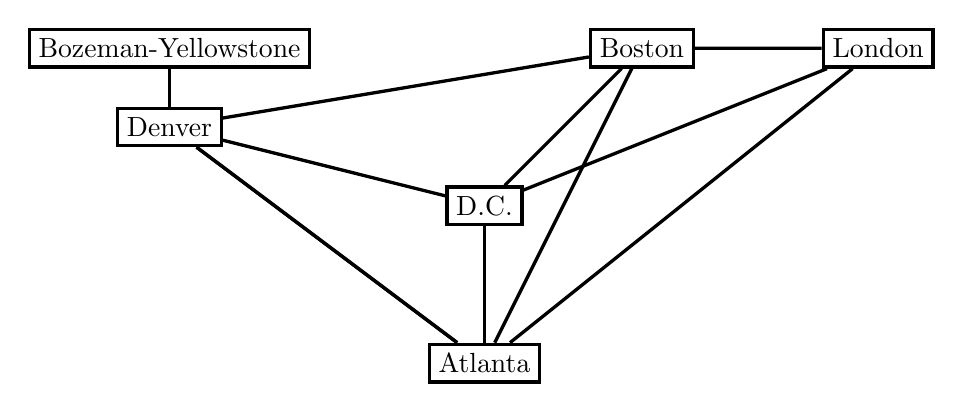
\begin{tikzpicture}[very thick,level/.style={sibling distance=70mm/#1}]
\draw (0, 0) node[draw, shape=rectangle] (a) {D.C.};
\draw (-4, 1) node[draw, shape=rectangle] (b) {Denver};
\draw (0, -2) node[draw, shape=rectangle] (c) {Atlanta};
\draw (2, 2) node[draw, shape=rectangle] (d) {Boston};
\draw (5, 2) node[draw, shape=rectangle] (e) {London};
\draw (-4, 2) node[draw, shape=rectangle] (f) {Bozeman-Yellowstone};
\draw (a) -- (b) -- (c) -- (d) -- (e);
\draw (b) -- (f);
\draw (c) -- (b);
\draw (a) -- (d);
\draw (b) -- (d);
\draw (a) -- (c);
\draw (c) -- (e);
\draw (a) -- (e);
\end{tikzpicture}
\end{center}

Our connections between our cities in the graph represent only direct connections between
cities, but from our diagram, we can still see it is possible to travel between any two
cities in our graph.

\textbf{Neither the exact position of each city nor the way that we draw the connection between the cities
matters.} The following is an equivalent graph:

\begin{center}
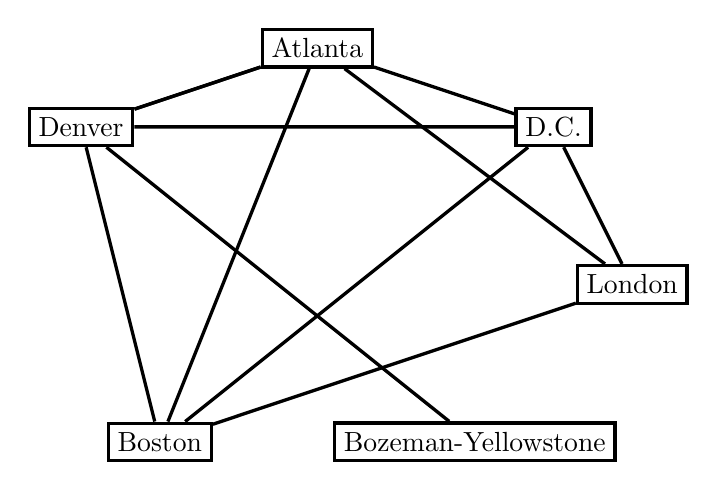
\begin{tikzpicture}[very thick,level/.style={sibling distance=70mm/#1}]
\draw (4, 3) node[draw, shape=rectangle] (a) {D.C.};
\draw (-2, 3) node[draw, shape=rectangle] (b) {Denver};
\draw (1, 4) node[draw, shape=rectangle] (c) {Atlanta};
\draw (-1, -1) node[draw, shape=rectangle] (d) {Boston};
\draw (5, 1) node[draw, shape=rectangle] (e) {London};
\draw (3, -1) node[draw, shape=rectangle] (f) {Bozeman-Yellowstone};
\draw (a) -- (b) -- (c) -- (d) -- (e);
\draw (b) -- (f);
\draw (c) -- (b);
\draw (a) -- (d);
\draw (b) -- (d);
\draw (a) -- (c);
\draw (c) -- (e);
\draw (a) -- (e);
\end{tikzpicture}
\end{center}

The only characteristics of a graph we care about are the objects (in this case, cities) themselves, which we'll call \textit{vertices},
and the connections joining the objects, which we'll call \textit{edges}.

\section{Formal Definition of a Graph}

We now have the background necessary to present the mathematical definition of a graph:

\begin{definition}
\label{def:graph}
A \textit{graph} $G(V,E)$ consists of a set of vertices $V$ and a set of edges $E$. 

\begin{center}
\begin{tikzpicture}[very thick,level/.style={sibling distance=70mm/#1}]
\draw (0, 0) node [vertex] (A) {$A$};
\draw (2, 1) node [vertex] (B) {$B$};
\draw (2, -1) node  [vertex] (C) {$C$};
\draw (4, 0) node [vertex] (D) {$D$};
\draw (A) -- (B);
\draw (B) -- (C);
\draw (C) -- (D);
\draw (B) -- (D);
\draw (A) -- (C);
\draw (6, -1) node [vertex] (E) {$E$};
\draw (6, 1) node [vertex] (F) {$F$};
\draw (8, 1) node [vertex] (G) {$G$};
\draw (8, -1) node [vertex] (H) {$H$};
\draw (E) -- (F) -- (G) -- (H) -- (F);
\draw (10, 0) node[vertex] (I) {$I$};
\draw (12, 0) node[vertex] (J) {$J$};
\draw (I) -- (J);
\end{tikzpicture}
\end{center}
\end{definition}

\begin{definition}
\label{def:edge}
An \textit{edge} is a collection of exactly two vertices. In the above graph, there is an edge
between $A$ and $B$, so $\{A, B\}$ is an edge. Note that $\{A,B\}$ is the same edge as $\{B,A\}$.
\end{definition}

\begin{definition}
\label{def:set}
A \textit{set} is a collection of any number of objects. In the above graph, we have the set of vertices
\[V=\{A, B, C, D, E, F, G, H, I, J\}.\]
We also have the set of edges
\[E=\{\{A,B\}, \{B,C\}, \{C,D\},\{B,D\},\{A,C\},\{E,F\},\{F,G\},\{G,H\},\{H,F\},\{I,J\} \}.\]
\end{definition}

\begin{definition}
\label{def:cardinality}
Given a set $A$, the cardinality $\abs{A}$ denotes the number of elements in $A$.
\end{definition}

\begin{problem} % problem 1
Evaluate $\abs{V}$ and $\abs{E}$ for the sets $V$ and $E$ in Definition \ref{def:set}, the definition of the set.
Note that $\{A,B\}$ counts as one single edge.
\end{problem}

\begin{solution}
Answer: $\abs{V} = \abs{E} = \boxed{10}$. \\
There are 10 vertices and 10 edges in the graph.
\end{solution}

\begin{problem} % 2
Draw any graph with 5 vertices and 8 edges.
\end{problem}

\begin{solution}
The following graph has 5 vertices and 8 edges.
\begin{center}
\begin{tikzpicture}[very thick,level/.style={sibling distance=70mm/#1}]
\draw (6, -1) node [vertex] (A) {$A$};
\draw (6, 1) node [vertex] (B) {$B$};
\draw (8, 1) node [vertex] (C) {$C$};
\draw (8, -1) node [vertex] (D) {$D$};
\draw (10, 0) node [vertex] (E) {$E$};
\draw (A) -- (B) -- (C) -- (D) -- (A) -- (C) -- (E) -- (D) -- (B);
\end{tikzpicture}
\end{center}
\end{solution}

\begin{definition}
\label{def:clique}
A \textit{clique} is a graph such that there is exaclty one edge covering every pair of distince vertices in the graph.
We denote a clique of $n$ vertices as $K_n$.
Pictured is a clique of 4 vertices, or $K_4$.
\begin{center}
\begin{tikzpicture}[very thick,level/.style={sibling distance=70mm/#1}]
\draw (6, -1) node [vertex] (A) {$A$};
\draw (6, 1) node [vertex] (B) {$B$};
\draw (8, 1) node [vertex] (C) {$C$};
\draw (8, -1) node [vertex] (D) {$D$};
\draw (A) -- (B) -- (C) -- (D) -- (A);
\draw (A) -- (C);
\draw (B) -- (D);
\end{tikzpicture}
\end{center}
\end{definition}

\begin{problem}
Solve each of the following:
\begin{enumerate}[label=(\alph*)]
\item How many edges are in the clique of 4 vertices, $K_4$?
\item How many edges are in the clique of 5 vertices, $K_5$?
\item In terms of $n$, how many edges are in the clique of $n$ vertices, $K_n$, where $n$ is any positive integer?
\end{enumerate}
\end{problem}

\begin{solution} 
The number of edges in a clique are as follows:
\begin{enumerate}[label=(\alph*)]
\item $K_4$ has \boxed{6} edges: $\{A, B\}$, $\{A, C\}$, $\{B, C\}$, $\{A, D\}$, $\{B, D\}$, $\{C, D\}$.
\item $K_5$ has \boxed{10} edges: $\{A, B\}$, $\{A, C\}$, $\{B, C\}$, $\{A, D\}$, $\{B, D\}$, $\{C, D\}$, $\{A, E\}$, $\{B, E\}$, $\{C, E\}$, $\{D,E\}$.
\item In general, $K_n$ has
\[\binom{n}{2} = \boxed{\frac{n \cdot (n - 1)}{2}}\]
edges. \\
We need to count the total number of possible ways to choose two different vertices from $n$ total vertices. We have $n$ ways to choose the first vertex
and $n - 1$ ways to choose the second vertex, but the order in which we choose the vertices doesn't matter (that is, $\{A,B\}$ represents the same edge
as $\{B, A\}$), so we must divide by 2 to get the correct answer of $\frac{n \cdot (n - 1)}{2}$.
\end{enumerate}
\end{solution}

\end{document}

